\section*{Learning Objectives}

\begin{itemize}
\item Checking linear independence vs determining the number of linearly independent vectors
\item  What is LDLT?
\item  How can it be used to count the number of linearly independent vectors?
\item Debugging, or finding and fixing errors in your code.
\end{itemize}

\section*{Outcomes} 
\begin{itemize}
\item Applying LU for checking linear Independence
\item Matrices of the form $A^\top A$ can always be factored as $ L\cdot D \cdot L^\top$, where $L$ is uni-lower triangular and $D$ is diagonal with non-negative entries
\item Counting the number of linearly independent vectors in a set via LDLT
\item Finding a maximal subset of linearly independent vectors
\end{itemize}

\vspace*{1cm}

\textbf{Either download Lab5 from our Canvas site or open up a Jupyter notebook so that you can enter code as we go. It is suggested that you have line numbering toggled on.}  

\newpage

We've covered most of the Julia coding that we need for ROB 101. This lab will focus on (a) using LU Factorization for checking if a set of vectors is linearly independent or not, and (b) presenting an enhanced version of LU Factorization for separating a set of vectors into a first group of linearly independent vectors and a second group of vectors that are dependent on the first group. The enhanced form of LU factorization goes by the name of LDLT Factorization or the Cholesky Factorization.\\



\section{Checking Linear Independence with LU}

From Chapter 7 of the ROB 101 Textbook,

\begin{tcolorbox}[sharp corners, colback=green!30, colframe=green!80!blue,
title=\textbf{Pro-tip! Linear Independence in a Nutshell}]
Consider the vectors in $\real^n$,
$$\left\{v_1=\begin{bmatrix} a_{11} \\ a_{21}\\ \vdots \\ a_{n1} \end{bmatrix},  v_2=\begin{bmatrix} a_{12} \\ a_{22}\\ \vdots \\ a_{n2} \end{bmatrix}, ...,  v_m=\begin{bmatrix} a_{1m} \\ a_{2m}\\ \vdots \\ a_{nm} \end{bmatrix} \right\},$$ 
and use them as the columns of a matrix that we call $A$,
\begin{equation}
\label{eq:MatrixFromLinearIndependence_proTipC}    
A=\left[\begin{array}{cccc} a_{11}& a_{12}& \cdots & a_{1m} \\
 a_{21}& a_{22}& \cdots & a_{2m}  \\
 \vdots & \vdots&  \ddots & \vdots \\
 a_{n1}& a_{n2}& \cdots & a_{nm} 
 \end{array}\right].
 \end{equation}
 The following statements are equivalent:
 \begin{itemize}
     \item  The set of vectors $ \{v_1, v_2, \ldots, v_m \} $ is linearly independent.
     \item The $m \times m$ matrix $A^\top \cdot A$ is invertible. 
     \item $\det(A^\top \cdot A) \neq 0$.
     \item For any LU Factorization $P \cdot (A^\top \cdot A) = L \cdot U$  of $A^\top A$, the $m \times m$ upper triangular matrix $U$ has no zeros on its diagonal.
 \end{itemize}
\end{tcolorbox}

\vspace*{.2cm}

Here is an implementation of the LU Factorization Algorithm. \\

\begin{lstlisting}[language=Julia,style=mystyle]
using LinearAlgebra
function myLU(M::Array{<:Number, 2})
    a, b = size(M)
    n=min(a,b)
    Temp = deepcopy(M)
    L = Matrix{Float64}(undef, a, n)
    U = Matrix{Float64}(undef, n, b)
    epsilon=1e-12
    P=zeros(a,a) + I
    for k = 1:n
        C = Temp[:,k] # k-th column
        R = Temp[k:k,:] # k-th row
        if maximum(abs.(C)) <= epsilon #column of zeros
            C=0.0*C
            C[k]=1.0
            Temp=Temp-C*R
            L[:,k]=C
            U[k:k,:]=R  
        else # put the biggest entry to the top
            ii=argmax( abs.(C) )
            nrow=ii[1] 
            # Do row permutations
            P[[k,nrow],:]=P[[nrow,k],:]
            Temp[[k,nrow],:]=Temp[[nrow,k],:]
            if k>1
                L[[k,nrow],:]= L[[nrow,k],:]
            end
            C = Temp[:,k] # k-th column
            pivot = C[k]
            C=C/pivot #normalize all entires by C[i]
            R = Temp[k:k,:] # k-th row
            Temp=Temp-C*R
            L[:,k]=C
            U[k:k,:]=R
        end
    end         
    return L, U, P
end
\end{lstlisting}
\textbf{Output} 
\begin{verbatim}
myLU (generic function with 1 method)
\end{verbatim}

We generate two matrices. One that we know will be be linearly dependent because we have four vectors in $\real^3$ and another we expect to be linearly independent because we have four random vectors in $\real^5$.\\

\begin{lstlisting}[language=Julia,style=mystyle]
using Random
Random.seed!(3141596)
A=randn(3,4)
B=randn(5,4)
\end{lstlisting}
\textbf{Output} 
\begin{verbatim}
5×4 Matrix{Float64}:
 -1.45267    0.0432641   0.562999    0.0499658
 -0.271694  -0.426124   -1.58141    -0.457054
  0.371157   1.99933    -0.0944284  -2.27898
  0.950984   1.19788    -0.588755    1.61326
  0.422272  -0.440388    1.13876    -0.70359
\end{verbatim}
Once again, we know that the columns of $A$ must be linearly dependent because we have four vectors in $\real^3$. If the four columns of $A$ were linearly independent, then $\real^3$ would have at least dimension four. But we know that $\real^3$ has dimension three, and hence the set of four vectors must be dependent. From the \textbf{Pro-tip!}, to evaluate (check) the linear independence of the columns of $A$, we can perform the LU factorization of $A^\top \cdot A$ and inspect the diagonal of $U$ for zeros.\\ 

\begin{lstlisting}[language=Julia,style=mystyle]
L, U, P = myLU(A'*A)
U
\end{lstlisting}
\textbf{Output} 
\begin{verbatim}
4×4 Matrix{Float64}:
 7.00075   6.54966   -2.93873    1.27537
 0.0      -0.446701  -0.0255008  0.928349
 0.0       0.0        0.386878   0.56443
 0.0       0.0        0.0        1.05471e-15
\end{verbatim}

$U[4,4]=1.0547$1e-15 is numerically zero and thus we see that the columns of $A$ are \textbf{linearly dependent}. Just for the fun of it, we'll give a function that ``cleans up'' the almost zero entries of a matrix or vector and makes them equal to 0.0. We'll set the tolerance as 1e-10\\

\begin{lstlisting}[language=Julia,style=mystyle]
function cleanUp(A,tol=1e-10)
    # Zero out small entries of a matrix or vector
    B=copy(A)
    indicesSmall=findall(x->x<tol, abs.(B))
    B[indicesSmall]=0.0*B[indicesSmall]
return B
end
#
cleanUp(U)
\end{lstlisting}
\textbf{Output} 
\begin{verbatim}
4×4 Matrix{Float64}:
 7.00075   6.54966   -2.93873    1.27537
 0.0      -0.446701  -0.0255008  0.928349
 0.0       0.0        0.386878   0.56443
 0.0       0.0        0.0        0.0
\end{verbatim}
Now, there is clearly a zero on the diagonal of $U$ and hence the columns of $A$ are not linearly independent. \\

The function \texttt{cleanUP} uses the Julia function \texttt{findall} that allows you to find the indices of all values of an array that satisfy a criterion that you set. \\

\begin{lstlisting}[language=Julia,style=mystyle]
? findall
\end{lstlisting}
\textbf{Output} 
\begin{verbatim}
It's super long. You can check it out yourself if interested. 
\end{verbatim}

Now we check the matrix $B$,

\begin{lstlisting}[language=Julia,style=mystyle]
L, U, P = myLU(B'*B)
cleanUp(U)
\end{lstlisting}
\textbf{Output} 
\begin{verbatim}
4×4 Matrix{Float64}:
 3.40451  1.74819  -0.50227    0.442818
 0.0      4.91194  -0.439397  -2.34454
 0.0      0.0       4.35675   -0.929314
 0.0      0.0       0.0        7.12791
\end{verbatim}

For the matrix $B$, there are no zeros on the diagonal of $U$ and hence the columns of $B$ are linearly independent.\\

\section{LU is a Suboptimal Tool for Determining the Number of Linearly Independent Vectors in a Set}

A more advanced question than linear independence is \textbf{how many linearly independent vectors} are there in a given set of vectors? An even more advanced question is \textbf{which ones are they?} In this section, we'll provide a first treatment of these questions. \\

We consider the $5 \times 5$ matrix 
\begin{equation}
A:= \left[
\begin{array}{rrrrr}
0.8814 & 1.1974 & 2.5033 & -1.8788 & -0.9375 \\
-0.4241 & 1.1761 & 2.1315 & -3.5430 & 0.8276 \\
1.0306 & -0.3120 & -0.3325 & 2.1482 & -1.4951 \\
-0.1551 & 2.9496 & 5.5761 & -7.6896 & -0.1905 \\
-1.2632 & -0.1046 & -0.5197 & -1.3970 & 0.7202 \\
\end{array}
\right]
\end{equation}

We check \texttt{myLU($A^\top \cdot A$)}.\\


\begin{lstlisting}[language=Julia,style=mystyle]
L, U, P = myLU(A'*A)
cleanUp(diag(U))
\end{lstlisting}
\textbf{Output} 
\begin{verbatim}
5-element Vector{Float64}:
  5.018367341067237
 26.544273902523273
 -0.0
 -0.0
 -0.0
\end{verbatim}

We conclude that the columns of $A$ are not linearly independent. Now, we ask, how many of the columns of $A$ can we choose and still have a linearly independent set? Looking at the diagonal of $U$, you may be tempted to say two! \textbf{But you would be wrong!}

\begin{figure}[htb]%
	\centering
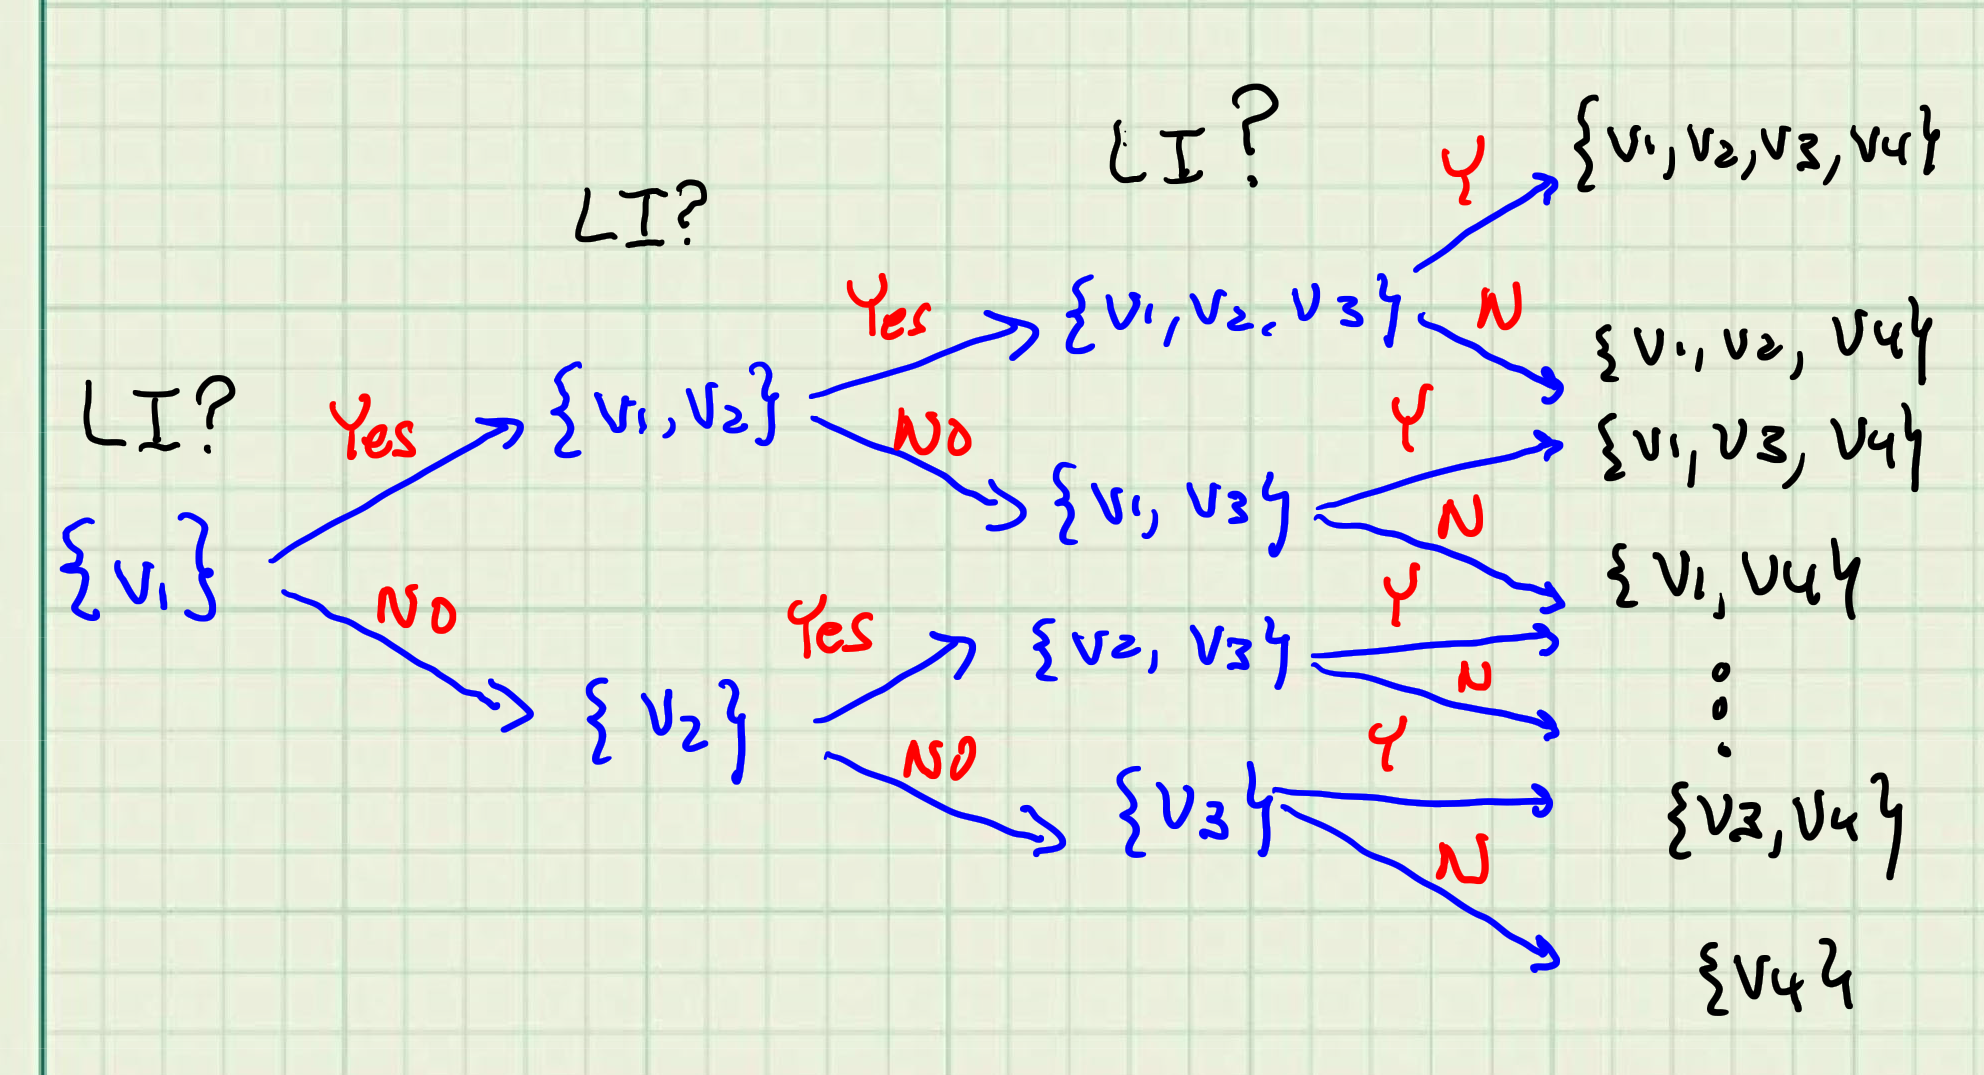
\includegraphics[width=0.88\columnwidth]{graphics/Chap05/NumberLinearIndependentVectorsInSet.png}
\caption[]{Checking linear independence from left to right. You could also start from the right and go to the left, or you could start in the middle and proceed to the two ends. You just need to do an organized search of the vectors!}
    \label{fig:NumberLinearlyIndependentVectors}
\end{figure}

In the following, we will implement the process indicated in Fig.~\ref{fig:NumberLinearlyIndependentVectors}, which shows one way to systematically check linear independence of a set of vectors to arrive at a maximal subset of linearly independent vectors. Along the way, we'll also keep track of the indices of the vectors that are linearly independent.\\ 

\begin{lstlisting}[language=Julia,style=mystyle]
function mySearchRoutine4NumIndepVectors(A,atol=1e-10)
    nRowsA, nColsA = size(A)
    V=Matrix{Float64}(undef, nRowsA, 0) # create an empty matrix
                                    # for storing independent vectors
    numIndVectors= 0
    indices = Vector{Int64}(undef, 0)  # create an empty vector for storing
                                # the indices of independent vectors
    for i = 1 : nColsA
        Temp=[V  A[:,i]]
        L, U, P = myLU(Temp'*Temp)
        minDiagU = minimum(abs.(diag(U)))
        # If minDiagU > atol, then U is invertible and hence the columns
        # of Temp are linearly independent
        if minDiagU > atol
            numIndVectors = numIndVectors + 1
            V = Temp
            indices = [indices; i] # keep track of indep vectors
        end
    end
    return numIndVectors, V, indices
end
\end{lstlisting}
\textbf{Output} 
\begin{verbatim}
mySearchRoutine4NumIndepVectors (generic function with 2 methods)
\end{verbatim}

We next show that $A$ has three linearly independent columns and we can choose them as the first, second, and fifth columns. \\

\begin{lstlisting}[language=Julia,style=mystyle]
numIndVectors, V, indices = mySearchRoutine4NumIndepVectors(A)
\end{lstlisting}
\textbf{Output} 
\begin{verbatim}
3, [0.8814395099307569 1.1974345124883454 -0.9375085811788099; -0.4241418472936163
1.1761409436174899 0.8276128787991263; … ; -0.15514669800915096 2.949627319800578
-0.1905215623370098; -1.2632013933716764 -0.10460087472162416 0.7201716618604121], 
[1, 2, 5])
\end{verbatim}

\begin{lstlisting}[language=Julia,style=mystyle]
numIndVectors
\end{lstlisting}
\textbf{Output} 
\begin{verbatim}
3
\end{verbatim}

\begin{lstlisting}[language=Julia,style=mystyle]
V
\end{lstlisting}
\textbf{Output} 
\begin{verbatim}
5×3 Matrix{Float64}:
  0.88144    1.19743   -0.937509
 -0.424142   1.17614    0.827613
  1.03061   -0.312031  -1.49514
 -0.155147   2.94963   -0.190522
 -1.2632    -0.104601   0.720172
\end{verbatim}

\begin{lstlisting}[language=Julia,style=mystyle]
indices
\end{lstlisting}
\textbf{Output} 
\begin{verbatim}
3-element Vector{Int64}:
 1
 2
 5
\end{verbatim}

Could we have made other choices for three linearly independent vectors? Absolutely. The following shows that we could have taken the last three vectors. 
\begin{lstlisting}[language=Julia,style=mystyle]
 numIndVectors, V, indices = mySearchRoutine4NumIndepVectors(A[:,3:5])
\end{lstlisting}
\textbf{Output} 
\begin{verbatim}
(3, [2.503340396444761 -1.8787774833565118 -0.9375085811788099; 2.1314687886946517
-3.5429649155470724 0.8276128787991263; … ; 5.576055157377987 -7.68964057029396
-0.1905215623370098; -0.5197147429767035 -1.3969985094856063 0.7201716618604121], 
[1, 2, 3])
\end{verbatim}

Could we have taken any three vectors? Let's check! We'll do a brute force search to find all combinations of three vectors that are linearly \textbf{dependent}, if any. Note that we can assume without loss of generality that $i < j < k$ when we consider three columns $\{A_i, A_j, A_k \}$ of $A$. Why? Because order does not change linear independence. \\

This code block outputs all combinations of three vectors that are linearly dependent.  \\

\begin{lstlisting}[language=Julia,style=mystyle]
for i = 1:3
    for j = i+1:5
        for k = j+1:5
             numIndVectors, V, indices = mySearchRoutine4NumIndepVectors(A[:,[i;j;k]])
            if numIndVectors < 3 
                @show [i;j;k]  # dependent columns              
            end
        end
    end
end
\end{lstlisting}
\textbf{Output}
\begin{verbatim}
[i; j; k] = [1, 2, 3]
[i; j; k] = [1, 2, 4]
[i; j; k] = [1, 3, 4]
[i; j; k] = [2, 3, 4]
\end{verbatim}

Once we know all combinations of columns of $A$ that are linearly dependent, we can deduce that the following sets of vectors are linearly independent.
\begin{itemize}
    \item  $\{A_1, A_2, A_5 \}$ 
    \item  $\{A_1, A_3, A_5 \}$ 
    \item  $\{A_2, A_3, A_5 \}$ 
    \item  $\{A_2, A_4, A_5 \}$ 
     \item  $\{A_3, A_4, A_5 \}$ 
\end{itemize}

\section{LDLT Factorization: A One-shot Means to Find Linearly Independent Vectors in a Set}

Once again, consider the vectors in $\real^n$,
$$\left\{v_1=\begin{bmatrix} a_{11} \\ a_{21}\\ \vdots \\ a_{n1} \end{bmatrix},  v_2=\begin{bmatrix} a_{12} \\ a_{22}\\ \vdots \\ a_{n2} \end{bmatrix}, ...,  v_m=\begin{bmatrix} a_{1m} \\ a_{2m}\\ \vdots \\ a_{nm} \end{bmatrix} \right\},$$ 
and use them as the columns of a matrix that we call $A$,
\begin{equation}
\label{eq:MatrixFromLinearIndependence_proTipC02}    
A=\left[\begin{array}{cccc} a_{11}& a_{12}& \cdots & a_{1m} \\
 a_{21}& a_{22}& \cdots & a_{2m}  \\
 \vdots & \vdots&  \ddots & \vdots \\
 a_{n1}& a_{n2}& \cdots & a_{nm} 
 \end{array}\right].
 \end{equation}

\begin{tcolorbox}[sharp corners, colback=green!30, colframe=green!80!blue,
title=\textbf{ {\Large \textcolor{red}{\bf Uber} Pro-Tip:} \large Number of Linearly Independent Vectors via an Enhanced LU Factorization}]
Assume that a set of vectors has been stacked to form the columns of an $n \times m$ matrix $A$ as in \eqref{eq:MatrixFromLinearIndependence_proTipC02}. \textbf{Fact:} The matrix $A^\top \cdot A$ always has an \textbf{LDLT Factorization}
\begin{equation}
    \label{eq:LDLTfactorization}
    P\cdot A^\top \cdot A \cdot P^\top = L\cdot D \cdot L^\top,
\end{equation}
where
\begin{itemize}
    \item $P$ is a (row) permutation matrix;
    \item $P^\top$, the transpose of $P$, permutes the columns of $A^\top A$;
    \item $L$ is uni-lower triangular and $L^\top$, the transpose of $L$, is therefore uni-upper triangular; and
    \item $D$ is diagonal and has non-negative entries.
\end{itemize}
\textcolor{red}{\bf Moreover,}
\begin{itemize}
    \item \textcolor{red}{\bf the number of linearly independent columns of $A$ is equal to the number of non-zero entries on the diagonal of $D$;} and, if we denote this number by $k$,
    \item  \textcolor{red}{\bf then for the version of the LDLT given below, the first $k$-columns of $A \cdot P^\top$ are linearly independent, and the remaining $(m-k)$-columns (if any) are linearly dependent on the first $k$ columns.} 
    \item Because the columns of $A\cdot P^\top$ are simply the columns of $A$ permuted by $P^\top$ (that is, re-ordered by the permutation matrix), \textcolor{red}{\bf the first $k$-columns of $A \cdot P^\top$ provide a selection of linearly independent columns of $A$}.
\end{itemize}

\end{tcolorbox}

While the derivation of this algorithm is not so different than what we did for the LU Factorization, we are still going to skip it. The main point is that matrices of the form $A^\top \cdot A$ always have an LDLT Factorization and, moreover, the diagonal of $D$ and the permutation matrix $P$ tell you everything you need to know about the linearly independent vectors that make up the columns of $A$. 

\begin{lstlisting}[language=Julia,style=mystyle]
function ldltROB101(A)
    epsilon = 1e-12
    M = A'*A
    n,m = size(A)
    Areduced = M
    L = Array{Float64,2}(undef,m,0)
    Id = zeros(m,m) + I
    P = Id    
    D=zeros(m,m)
    for i=1:m
        ii=argmax(diag(Areduced[i:m,i:m]))
        mrow=ii[1]+(i-1)
        if !(i==mrow)
            P[[i,mrow],:]=P[[mrow,i],:]
            Areduced[[i,mrow],:]=Areduced[[mrow,i],:]
            Areduced[:,[i,mrow]]=Areduced[:,[mrow,i]]
        end
        if (i>1)
            L[[i,mrow],:] = L[[mrow,i],:]
        end
        pivot=Areduced[i,i]
        if !isapprox(pivot,0,atol=epsilon)
            D[i,i]=pivot
            C=Areduced[:,i]/pivot
            L=[L C]
            Areduced=Areduced-(C*pivot*C')
        else
            L=[L Id[:,i:m]]
            break
        end
    end
    diagD=diag(D)
    return L,P,D,diagD
end
\end{lstlisting}
\textbf{Output} 
\begin{verbatim}
ldltROB101 (generic function with 1 method)
\end{verbatim}

We apply LDLT to the same $5 \times 5$ matrix we used before, namely
\begin{equation}
A:= \left[
\begin{array}{rrrrr}
0.8814 & 1.1974 & 2.5033 & -1.8788 & -0.9375 \\
-0.4241 & 1.1761 & 2.1315 & -3.5430 & 0.8276 \\
1.0306 & -0.3120 & -0.3325 & 2.1482 & -1.4951 \\
-0.1551 & 2.9496 & 5.5761 & -7.6896 & -0.1905 \\
-1.2632 & -0.1046 & -0.5197 & -1.3970 & 0.7202 \\
\end{array}
\right]
\end{equation} 

\begin{lstlisting}[language=Julia,style=mystyle]
L,P,D,diagD = ldltROB101(A)
@show diagD
D
\end{lstlisting}
\textbf{Output} 
\begin{verbatim}
diagD = [81.779373907533, 5.130204240478989, 0.7812212873817588, 0.0, 0.0]

5×5 Matrix{Float64}:
 81.7794  0.0     0.0       0.0  0.0
  0.0     5.1302  0.0       0.0  0.0
  0.0     0.0     0.781221  0.0  0.0
  0.0     0.0     0.0       0.0  0.0
  0.0     0.0     0.0       0.0  0.0
\end{verbatim}

We see immediately that we have three linearly independent vectors. Can we find easily a set of three columns of $A$ that are linearly independent? Yes. If we form $A \cdot P^\top$, the \textbf{Uber Pro-tip} tells us that then the first three columns will be linearly indepenent.  
\begin{lstlisting}[language=Julia,style=mystyle]
Abar=A*P'
\end{lstlisting}
\textbf{Output} 
\begin{verbatim}
5×5 Matrix{Float64}:
 -1.87878   2.50334   -0.937509   1.19743    0.88144
 -3.54296   2.13147    0.827613   1.17614   -0.424142
  2.14821  -0.332486  -1.49514   -0.312031   1.03061
 -7.68964   5.57606   -0.190522   2.94963   -0.155147
 -1.397    -0.519715   0.720172  -0.104601  -1.2632
\end{verbatim}

\begin{equation}
\overline{A}: = A \cdot P =\left[
\begin{array}{rrrrr}
-1.8788 & 2.5033 & -0.9375 & 1.1974 & 0.8814 \\
-3.5430 & 2.1315 & 0.8276 & 1.1761 & -0.4241 \\
2.1482 & -0.3325 & -1.4951 & -0.3120 & 1.0306 \\
-7.6896 & 5.5761 & -0.1905 & 2.9496 & -0.1551 \\
-1.3970 & -0.5197 & 0.7202 & -0.1046 & -1.2632 
\end{array}
\right]
\end{equation}

\begin{lstlisting}[language=Julia,style=mystyle]
numIndVectors, V, indices = myNumIndepVectors(Abar[:,1:3])
numIndVectors
\end{lstlisting}
\textbf{Output} 
\begin{verbatim}
3
\end{verbatim}

Which columns are they? From the permutation matrix, we can see that LDLT has selected the fourth, third, and fifth columns of $A$, $\{A_4, A_3, A_5 \}$. The order is not very important; it's a consequence of my implementation using the largest available pivot element at each pass of ``peeling the onion". \\

\begin{lstlisting}[language=Julia,style=mystyle]
P'
\end{lstlisting}
\textbf{Output} 
\begin{verbatim}
5×5 adjoint(::Matrix{Float64}) with eltype Float64:
 0.0  0.0  0.0  0.0  1.0
 0.0  0.0  0.0  1.0  0.0
 0.0  1.0  0.0  0.0  0.0
 1.0  0.0  0.0  0.0  0.0
 0.0  0.0  1.0  0.0  0.0
\end{verbatim}

Why this order? Once again, the way I wrote the LDLT algorithm, it permutes large elements on the diagonal of $A^\top \cdot A$ to the front.\\

Below is another version of a function to find the number of linear independent columns in a matrix, along with a specification of which columns to use.

\begin{lstlisting}[language=Julia,style=mystyle]
function myNumIndepVectors(A,myTol=1e-10)
    nRowsA, nColsA = size(A)
    V=Matrix{Float64}(undef, nRowsA, 0)
    L,P,D,diagD = ldltROB101(A)
    indicesLDLT=findall(x->x>myTol, diagD)
    numIndVectors = length(indicesLDLT)
    Ptrans = P'
    indices = Vector{Int64}(undef, numIndVectors)
    for i = 1:numIndVectors
            ind=argmax(Ptrans[:,i])
            indices[i]=ind[1] 
    end
    V=A[:,indices]
        
    return numIndVectors, V, indices
end
\end{lstlisting}
\textbf{Output} 
\begin{verbatim}
myNumIndepVectors (generic function with 2 methods)
\end{verbatim}


\begin{lstlisting}[language=Julia,style=mystyle]
numIndVectors, V, indices = myNumIndepVectors(A)
@show numIndVectors
@show indices
V
\end{lstlisting}
\textbf{Output} 
\begin{verbatim}
numIndVectors = 3
indices = [4, 3, 5]

5×3 Matrix{Float64}:
 -1.87878   2.50334   -0.937509
 -3.54296   2.13147    0.827613
  2.14821  -0.332486  -1.49514
 -7.68964   5.57606   -0.190522
 -1.397    -0.519715   0.720172
\end{verbatim}

\section{Debugging}

Here, we'll focus on the LU Function in Julia. Let's build a solver for $Ax=b$, when $A$ is square and invertible, and $A$ and $b$ have compatible sizes. We assume that the functions \texttt{forwardsub(L, b)} and \texttt{backwardsub(U, b)} have already been defined and error checked!\\

Let's include some packages and create some data.

\begin{lstlisting}[language=Julia,style=mystyle]
using LinearAlgebra
using Random
Random.seed!(2001)

A = randn(4,4)
b=randn(4,1);
\end{lstlisting}
\textbf{Output} 
Nothing due to the semicolon. We next write our first cut at a function to solve $Ax=b$



\begin{lstlisting}[language=Julia,style=mystyle]
function mySolver(A,b)
    L,U = lu(A)
    y =  forwardsub(L, b)
    x = backwardsub(U, y)
    return x
    return x
end      
\end{lstlisting}
\textbf{Output} 
\begin{verbatim}
mySolver (generic function with 1 method)
\end{verbatim}

We run our function and it seems to work because it does produce output!

\begin{lstlisting}[language=Julia,style=mystyle]
x =  mySolver(A,b)
\end{lstlisting}
\textbf{Output} 
\begin{verbatim}
4-element Vector{Float64}:
  0.2793805449608082
  2.6408473207373446
 -2.3464083290282343
 -0.7884784181920488
\end{verbatim}

About this time, you run one of our Friendly Checks and fail it. And you go, no way, my function works; it produces no errors. Look, I have actual output! So you post to Piazza, saying hey, I failed the Friendly Check! What's wrong with my code or with the Friendly Check itself? \\

\textcolor{blue}{\bf \large About this time of the semester, we start asking you to do some serious debugging yourself. So, let's do it.} \\

We first check if the solution is correct.

\begin{lstlisting}[language=Julia,style=mystyle]
norm(A*x-b)
\end{lstlisting}
\textbf{Output} 
\begin{verbatim}
1.5606151971175222
\end{verbatim}

Ooops! That is not close to zero. What's wrong? Well, on line 2 of your function, you called Julia's LU function with permutations! OH my gosh, you're right. Let's include the permutation matrix. So we do it.

\begin{lstlisting}[language=Julia,style=mystyle]
function mySolver(A,b)
    L,U, P = lu(A)
    y =  forwardsub(L, P*b)
    x = backwardsub(U, y)
    return x
    return x
end 
\end{lstlisting}
\textbf{Output} 
\begin{verbatim}
mySolver (generic function with 1 method)
\end{verbatim}

Everything looks good. We give it a whirl....and Julia is super unhappy. 

\begin{lstlisting}[language=Julia,style=mystyle]
x =  mySolver(A,b)
\end{lstlisting}
\textbf{Output} 
\begin{verbatim}
DimensionMismatch("matrix A has dimensions (4,1), matrix B has dimensions (4,1)")

Stacktrace:
  [1] _generic_matmatmul!(C::Matrix{Float64}, tA::Char, tB::Char, A::Matrix{Int64},
  B::Matrix{Float64}, _add::LinearAlgebra.MulAddMul{true, true, Bool, Bool})
    @ LinearAlgebra /buildworker/worker/package_linux64/build/usr/share/julia/stdlib/v1.6/
    LinearAlgebra/src/matmul.jl:814
  [2] generic_matmatmul!(C::Matrix{Float64}, tA::Char, tB::Char, A::Matrix{Int64}, 
  B::Matrix{Float64}, _add::LinearAlgebra.MulAddMul{true, true, Bool, Bool})
    @ LinearAlgebra /buildworker/worker/package_linux64/build/usr/share/julia/stdlib/
    v1.6/LinearAlgebra/src/matmul.jl:802
  [3] mul!
    @ /buildworker/worker/package_linux64/build/usr/share/julia/stdlib/
    v1.6/LinearAlgebra/src/matmul.jl:302 [inlined]
  [4] mul!
    @ /buildworker/worker/package_linux64/build/usr/share/julia/stdlib/
    v1.6/LinearAlgebra/src/matmul.jl:275 [inlined]
  [5] *
    @ /buildworker/worker/package_linux64/build/usr/share/julia/stdlib/
    v1.6/LinearAlgebra/src/matmul.jl:153 [inlined]
  [6] *
    @ /buildworker/worker/package_linux64/build/usr/share/julia/stdlib/
    v1.6/LinearAlgebra/src/matmul.jl:63 [inlined]
  [7] mySolver(A::Matrix{Float64}, b::Matrix{Float64})
    @ Main ./In[24]:3
  [8] top-level scope
    @ In[25]:1
  [9] eval
    @ ./boot.jl:360 [inlined]
 [10] include_string(mapexpr::typeof(REPL.softscope), mod::Module, 
 code::String, filename::String)
    @ Base ./loading.jl:1094
\end{verbatim}

We have a \textbf{DimensionMismatch("matrix A has dimensions (4,1), matrix B has dimensions (4,1)")} and it seems to be on line 3 of our function; we get that fron \texttt{@ Main ./In[14]:3}. So, we immediately suspect the function \texttt{backwardsub} has an error. However, we've used it many times before, and the line 
\begin{verbatim}
Stacktrace:
  [1] _generic_matmatmul!(C::Matrix{Float64}, tA::Char, tB::Char, A::Matrix{Int64}, 
  B::Matrix{Float64}, _add::LinearAlgebra.MulAddMul{true, true, Bool, Bool}) 
  \end{verbatim}
could tell us that we have a matrix multiplication problem. \\

Hence, let's use the \texttt{display} function to see what's up with that line of code. To save space here, we also include the function call on line 13. The output looks great, until it doesn't! 


\begin{lstlisting}[language=Julia,style=mystyle]
function mySolver(A,b)
    L,U,P = lu(A)
    display(L)
    display(U)
    display(P)
    display(P*b)
    y =  forwardsub(L, P*b)
    x = backwardsub(U, y)
    return x
    return x
end 

x =  mySolver(A,b)
\end{lstlisting}
\textbf{Output} 
\begin{verbatim}
4×4 Matrix{Float64}:
  1.0        0.0       0.0      0.0
 -0.374657   1.0       0.0      0.0
 -0.841164  -0.808034  1.0      0.0
 -0.207949  -0.591682  0.91447  1.0
4×4 Matrix{Float64}:
 -1.61455   0.810841   0.867077  -0.318762
  0.0      -1.66425   -0.958626  -1.56293
  0.0       0.0        0.811276  -1.17566
  0.0       0.0        0.0       -0.920034
4-element Vector{Int64}:
 1
 3
 4
 2
DimensionMismatch("matrix A has dimensions (4,1), matrix B has dimensions (4,1)")

Stacktrace:
  [1] _generic_matmatmul!(C::Matrix{Float64}, tA::Char, tB::Char, A::Matrix{Int64}, 
  B::Matrix{Float64}, _add::LinearAlgebra.MulAddMul{true, true, Bool, Bool})
    @ LinearAlgebra /buildworker/worker/package_linux64/build/usr/share/
    julia/stdlib/v1.6/LinearAlgebra/src/matmul.jl:814
  [2] generic_matmatmul!(C::Matrix{Float64}, tA::Char, tB::Char, A::Matrix{Int64}, 
  B::Matrix{Float64}, _add::LinearAlgebra.MulAddMul{true, true, Bool, Bool})
    @ LinearAlgebra /buildworker/worker/package_linux64/build/usr/share/julia/stdlib/
    v1.6/LinearAlgebra/src/matmul.jl:802
  [3] mul!
    @ /buildworker/worker/package_linux64/build/usr/share/julia/stdlib/
    v1.6/LinearAlgebra/src/matmul.jl:302 [inlined]
  [4] mul!
    @ /buildworker/worker/package_linux64/build/usr/share/julia/stdlib/
    v1.6/LinearAlgebra/src/matmul.jl:275 [inlined]
  [5] *
    @ /buildworker/worker/package_linux64/build/usr/share/julia/stdlib/v1.6/
    LinearAlgebra/src/matmul.jl:153 [inlined]
  [6] *
    @ /buildworker/worker/package_linux64/build/usr/share/julia/stdlib/
    v1.6/LinearAlgebra/src/matmul.jl:63 [inlined]
  [7] mySolver(A::Matrix{Float64}, b::Matrix{Float64})
    @ Main ./In[27]:6
  [8] top-level scope
    @ In[27]:13
  [9] eval
    @ ./boot.jl:360 [inlined]
 [10] include_string(mapexpr::typeof(REPL.softscope), mod::Module, 
 code::String, filename::String)
    @ Base ./loading.jl:1094

\end{verbatim}

From \texttt{\@ Main ./In[27]:6}, we see that we have an error on line 6. Also, looking at the displayed results, we note that the permutation matrix $P$ is a vector. Yikes! What is that all about? \textcolor{red}{\bf L,U, P = lu(A) returns, $L$, $U$, and the list of permutation indices, but not the permutation matrix.} \textbf{To obtain the matrix, you need to use }

\begin{lstlisting}[language=Julia,style=mystyle]
function mySolver(A,b)
    F = lu(A)
    U=F.U
    L=F.L
    P=F.P
    y =  forwardsub(L, P*b)
    x = backwardsub(U, y)
    return x
end 

x =  mySolver(A,b)
display(x)
norm(A*x- b)
\end{lstlisting}
\textbf{Output} 
\begin{verbatim}
4-element Vector{Float64}:
 -0.22542848860215622
 -2.222759959807066
  2.0136373165391372
  1.2566870405250985
  
7.2815418263566e-16
\end{verbatim}

\textbf{Bottom line:} We learned the following:
\begin{itemize}
    \item Just because a function runs with no errors does not mean it is correct. You, the creator of the function, need to run some simple tests to check the correctness of your function. Here, we simply applied the definition of $x$ being a solution to $Ax=b$, namely, $||Ax-b||=0$.

    \item There is useful information in the error messages. It takes practice to interpret them. At the very least, you can find the \textbf{line number} where things failed.

    \item Once you know approximately what is failing, insert a copious number of \texttt{display} or \texttt{@show} commands and compare what you see to what you expect. 

    \item Your checks can be much more focused than the generic Friendly Checks that we insert because you get to see where the error is occurring. 
\end{itemize}


\section{(Optional Read) Finding Counterexamples via Search}

How did we find a matrix where LU would mess up? We did a brute force search! 

\begin{lstlisting}[language=Julia,style=mystyle]
using LinearAlgebra
using Random
function CounterExample(atol=1e-10)
    # Set the seed because we want each student to obtain the same results
    Random.seed!(12121212)
    flag = 1
    N=5
    n=floor(Int,N/2)
    k=0
    while flag > 0
        # count how many times through the loop
        k=k+1
        Random.seed!(k)
        # Build a matrix A that has dependent column vectors
        B=randn(N,N-1)
        C=randn(n,n)
        A=[B[:,1:n] B[:,1:n]*C B[:,n+n:end]]
        # Apply LU to A'A
        F=lu(A'*A, check=false)
        diagU=diag(F.U)
        # Find all indices where the magnitue of the diagonal element is not too small
        indicesLU=findall(x->x>atol, abs.(diagU))
        # Now count them. This is LU's prediction of the number of linearly independent vectors
        NumLinIndepLU=length(indicesLU)
        # Apply LDLT to A'A; recall, our function forms A'*A
        L,P,D,diagD = ldltROB101(A)
         # Find all indices where the magnitue of the diagonal element is not too small
        indicesLDLT=findall(x->x>atol, diagD)
        # Now count them. This is LDLT's prediction of the number of linearly independent vectors
        NumLinIndepLDLT=length(indicesLDLT)
        # Check for a discrepancy in their reported number of linearly indep columns
        # and also, do not run forever. 1e5 seems like enough times to loop through random matrices
        if (NumLinIndepLDLT > NumLinIndepLU)||(k>1e5)
            return k, A, F, L, P, D, diagD
            flag=0
        end        
    end
end

function cleanUp(A,tol=1e-10)
    # Zero out small entries of a matrix or vector
    B=copy(A)
    indicesSmall=findall(x->x<tol, abs.(B))
    B[indicesSmall]=0.0*B[indicesSmall]
return B
end
\end{lstlisting}
\textbf{Output} 
\begin{verbatim}
CounterExample (generic function with 2 methods)
\end{verbatim}

\begin{lstlisting}[language=Julia,style=mystyle]
k, A, L, P, D, diagD = CounterExample()
println("It took us $k random matrices to generate an example where LU fails.")
println("Let's explore the example a bit.")
A
\end{lstlisting}
\textbf{Output} 
\begin{verbatim}
It took us 3 random matrices to generate an example where LU fails.

7×7 Matrix{Float64}:
  1.19156   -0.00197414  -0.51281   …  -1.06384    1.63691    0.633455
 -2.51973    1.00879     -1.58024       2.81498   -1.4239     0.68743
  2.07481    0.844223     0.511659     -3.14415    2.06393   -0.135094
 -0.97325    1.15807      0.733867     -0.118041  -1.31149    0.492822
 -0.101607  -0.475159    -1.40705       1.13615    0.756238   0.15671
 -1.54251   -0.244612    -0.707273  …   2.21941   -1.23019    1.23958
  0.100793   0.0718727   -1.1661        0.40164    0.923609  -1.21044
\end{verbatim}

% \begin{lstlisting}[language=Julia,style=mystyle]

% \end{lstlisting}
% \textbf{Output} 
% \begin{verbatim}

% \end{verbatim}

% \begin{lstlisting}[language=Julia,style=mystyle]

% \end{lstlisting}
% \textbf{Output} 
% \begin{verbatim}

% \end{verbatim}

% \begin{lstlisting}[language=Julia,style=mystyle]

% \end{lstlisting}
% \textbf{Output} 
% \begin{verbatim}

% \end{verbatim}

% \begin{lstlisting}[language=Julia,style=mystyle]

% \end{lstlisting}
% \textbf{Output} 
% \begin{verbatim}

% \end{verbatim}


% \begin{lstlisting}[language=Julia,style=mystyle]

% \end{lstlisting}
% \textbf{Output} 
% \begin{verbatim}

% \end{verbatim}

% \begin{lstlisting}[language=Julia,style=mystyle]

% \end{lstlisting}
% \textbf{Output} 
% \begin{verbatim}

% \end{verbatim}

% \begin{lstlisting}[language=Julia,style=mystyle]

% \end{lstlisting}
% \textbf{Output} 
% \begin{verbatim}

% \end{verbatim}

% \begin{lstlisting}[language=Julia,style=mystyle]

% \end{lstlisting}
% \textbf{Output} 
% \begin{verbatim}

% \end{verbatim}

% \begin{lstlisting}[language=Julia,style=mystyle]

% \end{lstlisting}
% \textbf{Output} 
% \begin{verbatim}

% \end{verbatim}

% \begin{lstlisting}[language=Julia,style=mystyle]

% \end{lstlisting}
% \textbf{Output} 
% \begin{verbatim}

% \end{verbatim}

% \begin{lstlisting}[language=Julia,style=mystyle]

% \end{lstlisting}
% \textbf{Output} 
% \begin{verbatim}

% \end{verbatim}

% \begin{lstlisting}[language=Julia,style=mystyle]

% \end{lstlisting}
% \textbf{Output} 
% \begin{verbatim}

% \end{verbatim}